\section{Experiments and Results }  \label{section:experimentresults}


\subsection{Experiments}

Our experiments are composed of 5 consecutive stages. Such as - (1) 2D matching between try-on cloth images and SMPL\cite{Loper2015SMPLAS} model silhouette, (2) reconstructing 3D cloth models from 2D input cloth images, (3) generating human body characteristics, (4) estimating 3D body models from 2D target human images and transferring 3D cloth models' information, and (5) blending rendered warped cloth images into the target human images. First, we generate A-posed SMPL\cite{Loper2015SMPLAS} model silhouettes for input cloth categories, i.e., long sleeve, sleeveless, short sleeve elbow, short sleeve half elbow, and short sleeve quarter elbow. Then, we use shape-context matching (SCM)\cite{BelongieMP02} between cloth input and processed template silhouette (Please see Figure \ref{fig:2DmatchingOfClothAndBody}). Thus, we apply thin-plate-spline (TPS)\cite{Bookstein1989PrincipalWT} transformation on the input cloth image and generate the 2D matched cloth images. This first stage is implemented in Matlab. Second stage is about generating necessary materials for other parts of the pipeline, i.e., generating target human properties e.g. 2D joints and segmentation parsing. We use couple of off-the-shelf methods for this purpose, OpenPose\cite{Cao2018OpenPoseRM} for estimating 2D joints of target humans, and Look-Into-Person (LIP)\cite{Liang2018LookIP} model for generating target human segmentation masks.

In the third stage, we load the template SMPL\cite{Loper2015SMPLAS} model and apply the 2D transformed cloth images as textures. This step is implemented in python, along with Chumpy\cite{loper2018chumpy} and OpenDR\cite{loper2014opendr}, similar to the implementation of Loper et al.\cite{Loper2015SMPLAS}. In the fourth stage, we reconstruct the 3D body model from the target human images following the implementation of Bogo et al.\cite{Bogo2016SMPLify}. Then, we transfer the cloth texture and model information into the target body models, which is also implemented in python, along with Chumpy\cite{loper2018chumpy} and OpenDR\cite{loper2014opendr}. Hence, we render the 3D deformed clothes, and generate the warped clothes and binary masks as in input for the blending network. 

Final stage is the deep-learning based blending network for try-on. We use the pytorch implementation of Wang et al.\cite{Wang2018TowardCI} and make our network improvements as mentioned in Section \ref{section:tryon}. We follow the same training procedures from CP-VTON\cite{Wang2018TowardCI}, for both geometric matching module (GMM) and try-on module (TOM). Finally, we use the trained try-on network as our blending step, where we use the 3D warped cloth images generated from the third stage as try-on input. Thus, we generate the final try-on image for the target try-on cloth and human image pairs. Please refer to Figure \ref{fig:pipeline} \& \ref{fig:clothtransfertryon} to see the full pipeline and flow of our approach.



\subsection{Results}


Figure \ref{fig:testresults} shows qualitative comparison results between the state-of-the-art image-based virtual try-on model CP-VTON\cite{Wang2018TowardCI} and our approach. As discussed in Section \ref{section:intro} and  \ref{section:classifiedeval}, CP-VTON\cite{Wang2018TowardCI} generates good try-on outputs when the target human images are mild posed and the target clothing is mono-colored. However, when it comes to warping try-on clothes with large deformations and preserving clothing characteristics in a more natural way, we argue that 2D image-based non-rigid deformations cannot really compete with 3D model based deformations. Therefore, we present the examples of the results from our approach, where the try-on clothes have detailed textures, and/or the target humans have big poses. Our proposed approach can realistically deform try-on clothes while preserving better clothing characteristics than 2D image-based approaches, and generating better final virtual try-on output as well.



\begin{figure*}[t]
   \centering
\begin{tabular}{cc|cc|cc}

Try-on cloth&Target human&GMM\cite{Wang2018TowardCI})&TOM\cite{Wang2018TowardCI})&Warped(Ours)&Try-on(Ours)\\

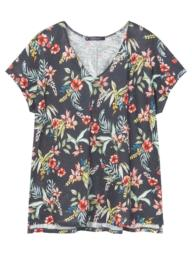
\includegraphics[width=2cm]{figures/cloth/002353_1.jpg}&
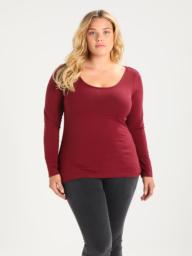
\includegraphics[width=2cm]{figures/image/007029_0.jpg}&
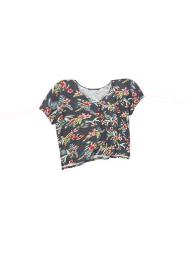
\includegraphics[width=2cm]{figures/cp-vton/warp-cloth/002353_1_007029_0.jpg}&
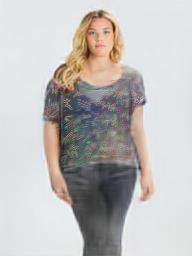
\includegraphics[width=2cm]{figures/cp-vton/try-on/002353_1_007029_0.jpg}&
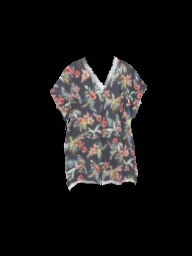
\includegraphics[width=2cm]{figures/c3dwfull/002353_1_007029_0.png}&
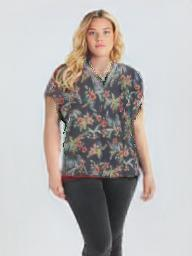
\includegraphics[width=2cm]{figures/try-on/002353_1_007029_0.jpg}\\

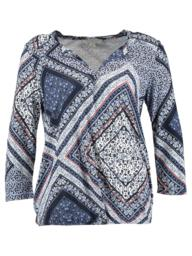
\includegraphics[width=2cm]{figures/cloth/016962_1.jpg}&
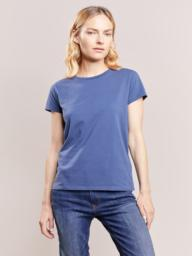
\includegraphics[width=2cm]{figures/image/005379_0.jpg}&
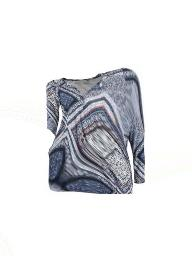
\includegraphics[width=2cm]{figures/cp-vton/warp-cloth/016962_1_005379_0.jpg}&
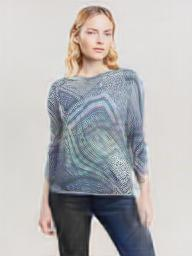
\includegraphics[width=2cm]{figures/cp-vton/try-on/016962_1_005379_0.jpg}&
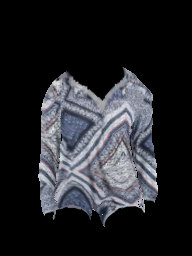
\includegraphics[width=2cm]{figures/c3dwfull/016962_1_005379_0.png}&
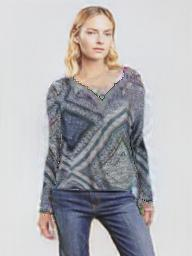
\includegraphics[width=2cm]{figures/try-on/016962_1_005379_0.jpg}\\

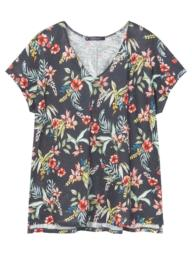
\includegraphics[width=2cm]{figures/cloth/002353_1.jpg}&
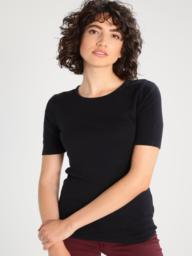
\includegraphics[width=2cm]{figures/image/019581_0.jpg}&
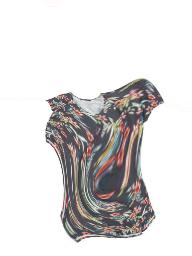
\includegraphics[width=2cm]{figures/cp-vton/warp-cloth/002353_1_019581_0.jpg}&
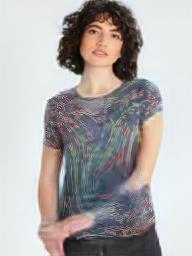
\includegraphics[width=2cm]{figures/cp-vton/try-on/002353_1_019581_0.jpg}&
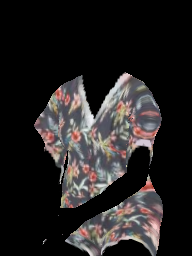
\includegraphics[width=2cm]{figures/c3dwfull/002353_1_019581_0.png}&
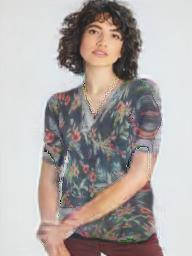
\includegraphics[width=2cm]{figures/try-on/002353_1_019581_0.jpg}\\

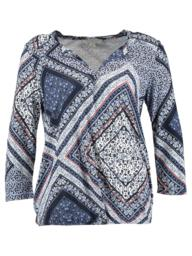
\includegraphics[width=2cm]{figures/cloth/016962_1.jpg}&
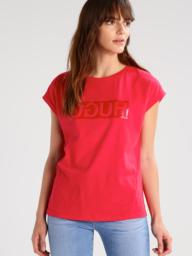
\includegraphics[width=2cm]{figures/image/019402_0.jpg}&
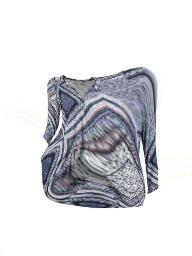
\includegraphics[width=2cm]{figures/cp-vton/warp-cloth/016962_1_019402_0.jpg}&
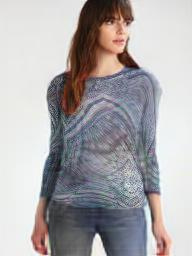
\includegraphics[width=2cm]{figures/cp-vton/try-on/016962_1_019402_0.jpg}&
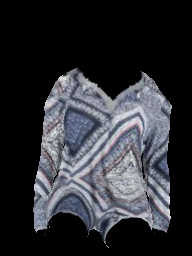
\includegraphics[width=2cm]{figures/c3dwfull/016962_1_019402_0.png}&
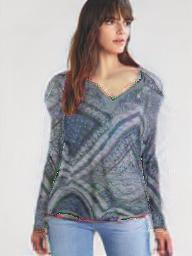
\includegraphics[width=2cm]{figures/try-on/016962_1_019402_0.jpg}\\

\end{tabular}

    \caption{Qualitative comparison between the baseline CP-VTON\cite{Wang2018TowardCI} and our approach. For each row, first pair of images are the inputs, try-on cloth and target human. Second pair is the warped cloth and final try-on results of CP-VTON\cite{Wang2018TowardCI}. And last pair includes the results of our approach; 3D reconstructed-deformed cloth, and the try-on results from the blending network.}
    \label{fig:testresults}
\end{figure*}




\subsection{Failure cases}

Although, our approach can reconstruct fashion clothes while preserving the clothing characteristics e.g. texture, color, shape realistically, there are cases where it fails to transfer cloth model to the target human and later in try-on. Especially the cases where SMPLify\cite{Bogo2016SMPLify} optimizations are mismatched. Additionally, as mentioned in Section \ref{section:tryon}, due to differences in training data and testing data of try-on/blending network, final try-on outputs gets worse. Figure \ref{fig:failurecases} shows few sample results of the failure cases in our methods. To improve our pipeline, we argue that more optimized and better algorithm for estimating 3D body model is needed. Also for mismatches in try-on network datasets, we can think of training with 3D warped clothes' dataset for further improvements.



\begin{figure*}
   \centering
\begin{tabular}{cccc}

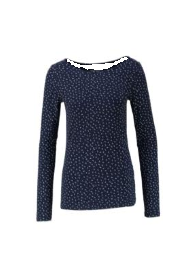
\includegraphics[width=1cm]{figures/c2dw/000118_1.png}&
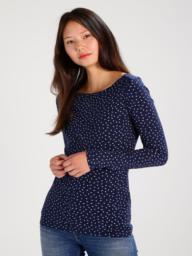
\includegraphics[width=1cm]{figures/image/000118_0.jpg}&
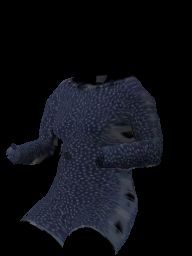
\includegraphics[width=1cm]{figures/c3dwfull/000118_1_000118_0.png}&
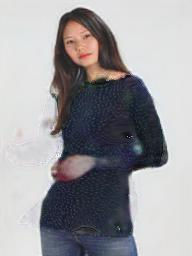
\includegraphics[width=1cm]{figures/try-on/000118_1_000118_0.jpg}\\

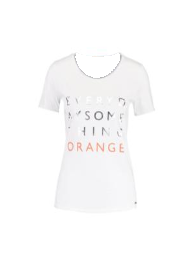
\includegraphics[width=1cm]{figures/c2dw/004508_1.png}&
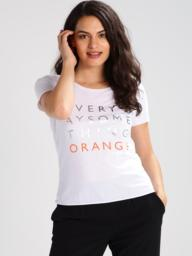
\includegraphics[width=1cm]{figures/image/004508_0.jpg}&
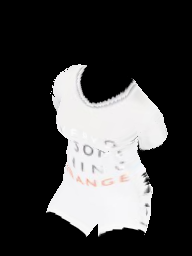
\includegraphics[width=1cm]{figures/c3dwfull/004508_1_004508_0.png}&
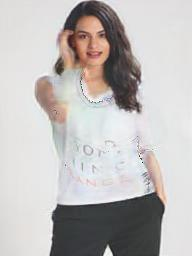
\includegraphics[width=1cm]{figures/try-on/004508_1_004508_0.jpg}\\

Cloth(2D)&Target&Cloth(Warped)&Try-on\\

\end{tabular}

    \caption{Failure cases}
    \label{fig:failurecases}
    
\end{figure*}



